\section{Matriz de Transição}

Dizemos que $A$ é uma matriz de transição, se $A = (a_{ij})_{1 \leq i,j \leq N}$ uma matriz quadrada de ordem $N$ tal que $a_{ij} \in \lbrace 0, 1 \rbrace$ para todo $1 \leq i,j \leq N$.
Se $A$ é uma matriz de transição, definimos o conjunto $\Sigma_A$ por
$$\Sigma_A = \lbrace (x_0 \, x_1 \, x_2 \, \dots) \in \Sigma_N : a_{x_k x_{k+1}} = 1 \text{ para todo } k \geq 0 \rbrace.$$
Observe que se $x \in \Sigma_A$, então $\sigma(x) \in \Sigma_A$.
Desse modo, podemos definir a função $\sigma_A: \Sigma_A \to \Sigma_A$ como sendo a restrição de $\sigma$ em $\Sigma_A$.

\begin{proposition}
$\Sigma_A$ é um subconjunto fechado de $\Sigma_N$.
\end{proposition}

\begin{proof}
Seja $\lbrace x_n \rbrace_{n=0}^{\infty}$ uma sequência de elementos em $\Sigma_A$ convergente para $x \in \Sigma_N$.
Vamos mostrar que $x \in \Sigma_A$.

Se $x = (\xi_0 \, \xi_1 \, \xi_2 \, \dots)$ e $x \notin \Sigma_A$, então existe $k \geq 0$ tal que $a_{\xi_k \xi_{k+1}} = 0$. Por outro lado, pela definição de convergência, existe $n_0 \geq 0$ tal que $d(x_{n_0}, x) < \frac{1}{N^{k+1}}$ e, portanto, as $k+2$ primeiras entradas de $x$ e $x_{n_0}$ são iguais. Escrevendo $x_{n_0} = (\eta_0 \, \eta_1 \, \eta_2 \, \dots)$, concluímos que $a_{\eta_k \eta_{k+1}} = a_{\xi_k \xi_{k+1}} = 0$, o que é um absurdo pois $x_{n_0} \in \Sigma_A$.
\end{proof}

No restante dessa seção vamos estudar a dinâmica da função quadrática $h_\mu(x) = \mu x(1-x)$, onde o parâmetro $\mu = 3.839$ está fixado. Será omitido $\mu$ na notação da função e escreveremos apenas $h$.

Se $a = 0.149888$, $\varepsilon = 10^{-3}$ e $I = (a - \varepsilon, a + \varepsilon)$, então é possível mostrar que $h^3(I) \subset I$ e $|D h^3(I)| < 1$ e, portanto, o intervalo $I$ possui um ponto periódico atrator de $h$ de período principal $3$. Se $a_1$, $a_2$ e $a_3$ são os elementos dessa órbita em ordem crescente, então
$$a_1 \simeq 0.149888 \text{, } \, a_2 \simeq 0.489149 \, \text{ e } \, a_3 \simeq 0.959299.$$
Pelo Teorema de Sharkovsky, $h$ possui infinitos pontos periódicos. Além disso, pelo Teorema de Singer, essa é a única órbita atratora de $h$.

De modo análogo, concluímos que $h$ possui outra órbita de tamanho $3$. Se $b_1$, $b_2$ e $b_3$ são os elementos dessa órbita em ordem crescente, então
$$b_1 \simeq 0.169040 \text{, } \, b_2 \simeq 0.539247 \,  \text{ e } \, b_3 \simeq 0.953837.$$

Observando o gráfico de $h^3$, concluímos que para cada $b_i$, existe $b'_i$ no lado oposto de $b_i$ em relação ao ponto $a_i$ tal que $h^3(b'_i) = b_i$. Defina $A_1 = (b'_1, b_1)$, $A_2 = (b'_2, b_2)$ e $A_3 = (b_3, b'_3)$. Cada $A_i$ é exatamente o intervalo maximal contendo $a_i$ utilizado na demonstração do Teorema de Singer.

\begin{center}
%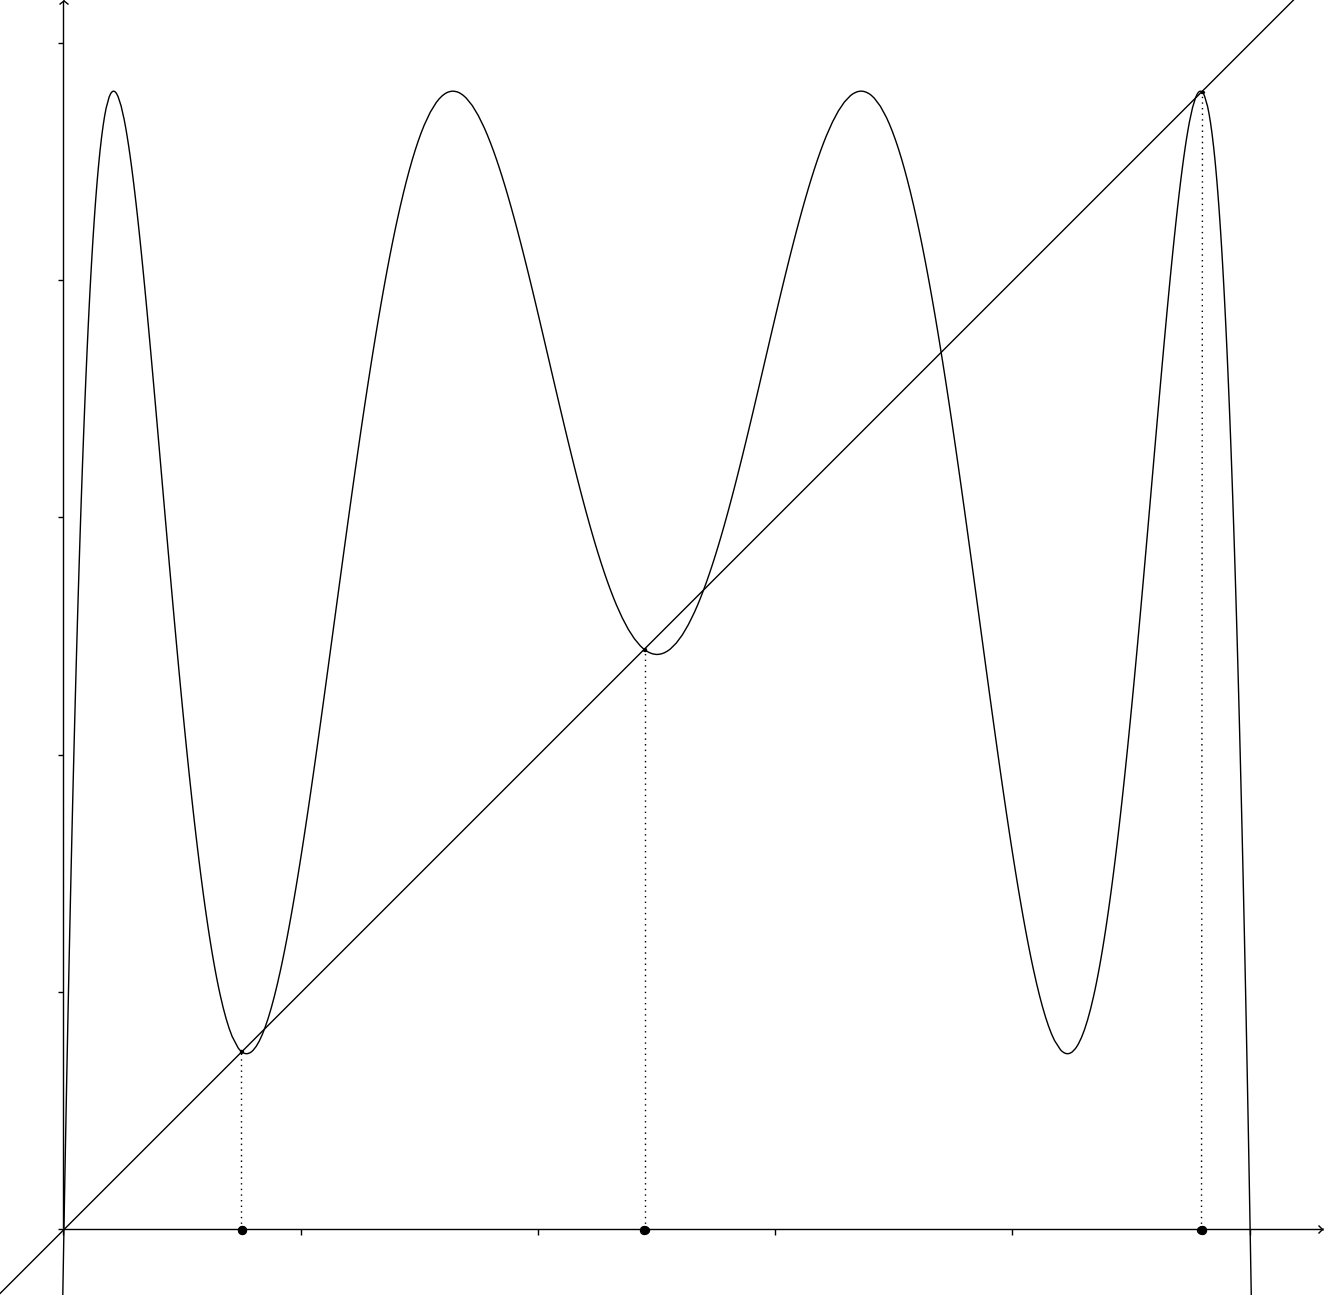
\includegraphics[scale=0.25]{images/f.png}
{\small \textbf{Figura:} Gráfico de $h^3$ com os pontos $a_1$, $a_2$ e $a_3$ assinalados.}
\end{center}

Sendo $h^3$ simétrica em relação ao ponto $\frac{1}{2}$, temos que $h(b'_2) = h(b_2) = b_3$.
Além disso, podemos observar que $h(b'_1) = b'_2$ e $h(b'_3) = b'_1$ e, portanto, $h$ mapeia de forma monótona $A_1$ em $A_2$ e $A_3$ em $A_1$. Observando que o máximo de $h$ em $A_2$ é $h( \frac{1}{2}) = 0.95975 < b'_3$, concluímos que $h(A_2) \subset A_3$.

Sabemos que se $x \notin [0, 1]$, então $\lim_{n \to \infty} h^n(x) = -\infty$.
Além disso, o único ponto periódico em $A_i$ é $a_i$ e todos os pontos em $A_i$ tendem para a órbita de $a_i$.
Desse modo, todos os outros pontos periódicos de $h$ residem no complemento de $A_1 \cup A_2 \cup A_3$ em $[0, 1]$, que é formado por quatro intervalos fechados. Sejam $J_0 = [0, b'_1]$, $J_1 = [b_1, b'_2]$, $J_2 = [b_2, b_3]$ e $J_3 = [b'_3, 1]$ tais intervalos. A Proposição a seguir nos permite dizer mais.

\begin{proposition}
Se $x \notin \lbrace 0, a_1, a_2, a_3 \rbrace$ é um ponto periódico de $h$, então $x \in J_1 \cup J_2$.
\end{proposition}

\begin{proof}
Observando que $h$ é monótona em cada $J_k$, temos que $h(J_0) = J_0 \cup A_1 \cup J_1$, $h(J_1) = J_2$, $h(J_2) = J_1 \cup A_2 \cup J_2$ e $h(J_3) = J_0$. Desse modo, se $x \in I_1 \cup J_2$ é periódico, então órbita de $x$ permanece em $J_1 \cup J_2$.

Por outro lado, se $x \in J_0 - \lbrace 0 \rbrace$, existe um menor $n \geq 1$ tal que $h^n(x) \notin J_0$. Se $h^n(x) \in A_1$, então $x$ não pode ser periódico, pois o único ponto periódico de $A_1$ é $a_1$.
Se $h^n(x) \in J_1$, então $x$ não pode ser periódico, pois caso contrário a órbita de $x$ estaria contida em $J_1 \cup J_2$ e nunca retornaria para $J_0$.
Finalmente, se $x \in J_3$, então $h(x) \in J_0$ e a análise segue de maneira análoga.
\end{proof}

Seja $\Lambda$ o conjunto dado por
$$\Lambda = \lbrace x \in J_1 \cup J_2 : h^n(x) \in J_1 \cup J_2 \text{ para todo } n \geq 1 \rbrace.$$
Pela Proposição anterior, todos os pontos periódicos de $h$ estão em $\Lambda$, com exceção dos pontos $0$, $a_1$, $a_2$ e $a_3$.

\begin{lemma}
Existe $n_0 \geq 1$ tal que $|D h^n(\Lambda)| > 1$ para todo $n \geq n_0$.
\end{lemma}

\begin{proof}
Inicialmente, podemos observar graficamente que $|D h(J_1 \cup J_2)| \geq \nu$ para algum $\nu \in (0, 1)$.
Podemos observar também que o subconjunto de $J_1 \cup J_2$ no qual $|D h^3|$ é menor que ou igual à $1$ é formado por três intervalos fechados e que cada um desses intervalos possui intersecção vazia com $\Lambda$ e, portanto, $|D h^3(\Lambda)| \geq \lambda$ para algum $\lambda > 1$.

Por fim, sejam $x \in \Lambda$ e $K \geq 1$ tal que $\nu^2 \lambda^K > 1$. Se $n_0 = 3K$ e $n \geq n_0$, podemos escrever $n = 3L + \alpha$, onde $L \geq K$ e $0 \leq \alpha \leq 2$. Desse modo, se $\alpha = 0$, então $ |D h^n(x)| = |D h^{3L}(x)|
\geq \lambda^L > 1$; se $\alpha = 1$, então $|D h^n(x)| = |D h(h^{3L}(x))| |D h^{3L}(x)| \geq \nu \lambda^L > 1$; e se $\alpha = 2$, então $|D h^n(x)| = |D h(h^{3L+1}(x))| |D h(h^{3L}(x))| |D h^{3L}(x)| \geq \nu^2 \lambda^L > 1$.
\end{proof}

\begin{lemma}
$\Lambda$ não contém intervalos.
\end{lemma}

\begin{proof}
Suponha que exista $[a, b] \subset \Lambda$. Utilizando notação do Lema anterior, seja $n \geq n_0$ tal que $\nu^{n_0} \lambda^{n - n_0} (b - a) > 1$. Pelo TVM, existe $c \in (a, b)$ tal que
\begin{align*}
|h^n(b) - h^n(a)| & = |D h^n(c)|(b-a) \\
& = \prod_{k=0}^{n_0-1} |D h(h^k(c))| \prod_{k=n_0}^{n-1} |D h(h^k(c))| (b-a) \\
& \geq \nu^{n_0} \lambda^{n-n_0} (b-a) > 1 \\
\end{align*}
e, portanto, $h^n(a)$ ou $h^n(b)$ não é elemento de $[0,1]$, o que é um absurdo.
\end{proof}

Para as demonstrações dos próximos resultados, vamos considerar a matriz de transição
$$A =
\begin{pmatrix}
0 & 1 \\
1 & 1 \\
\end{pmatrix}.$$
Seja $S: \Lambda \to \Sigma_A$ a função dada por $S(x) = (x_0 \, x_1 \, x_2 \, \dots)$, onde $x_k = 1$ se $h^k(x) \in J_1$ e $x_k = 2$ se $h^k(x) \in J_2$ para todo $k \geq 0$. Observe que $S$ está bem definida, pois $h(J_1) = J_2$ e $h(J_2) \subset J_1 \cup J_2$ e, portanto, $a_{x_k x_{k+1}} = 1$ para todo $k \geq 0$. 

\begin{theorem}
$h|_\Lambda$ e $\sigma_A$ são topologicamente conjugadas por $S$.
\end{theorem}
